\documentclass[10pt]{beamer}

\mode<presentation>
{
  \usetheme{Madrid}
  \usecolortheme{default}
  \usefonttheme{serif}
  \setbeamertemplate{navigation symbols}{}
  \setbeamertemplate{caption}[numbered]
  \setbeamertemplate{bibliography item}{\insertbiblabel}
}

\usepackage[english]{babel}
\usepackage[utf8x]{inputenc}
\usepackage[version=3]{mhchem}

\usepackage{pgfpages}
\usepackage{xcolor}
\usepackage{esvect}
\usepackage{graphicx}
\usepackage[compatibility=false]{caption}
\usepackage{subcaption}
\usepackage{soul} % for higglighting
\usepackage{verbatim} % comment blocks
\usepackage[font={footnotesize}]{caption} % customize caption size
\usepackage{appendixnumberbeamer} % to avoid numbering the reference slides
\usepackage{empheq}
\usepackage{xcolor}
\usepackage{multirow}
\usepackage{appendixnumberbeamer}
\newcommand{\boxedeq}[2]{\begin{empheq}[box={\fboxsep=6pt\fbox}]{align}\label{#1}#2\end{empheq}}




\pgfpagesuselayout{resize to}[%
  physical paper width=8in, physical paper height=6in]

\AtBeginSection[]
{
  \begin{frame}
    \frametitle{Table of Contents}
    \tableofcontents[currentsection]
  \end{frame}
}

\title[Multiphysics Coupling]{Preliminary Coupling of OpenMC and Nek5000 Within the MOOSE Framework}
\author[Novak, Romano, et. al]{A.~J.~ Novak\inst{1}, P.~K.~Romano\inst{2}, B.~Wendt\inst{3}, R.~Rahaman\inst{2}, E.~Merzari\inst{2}, C.~Permann\inst{4}, R.~C.~Martineau\inst{4}, L.~Kerby\inst{3,4}, R.~N.~Slaybaugh\inst{1}}
\institute[]
{
	\inst{1}
	Department of Nuclear Engineering\\
	University of California, Berkeley
	\and
	\inst{2}
	Argonne National Laboratory
	\and
	\inst{3}
	Idaho State University
	\and
	\inst{4}
	Idaho National Laboratory
}
\date[PHYSOR 2018]{April 25, 2018}

\begin{document}

\begin{frame}
  \titlepage
\end{frame}

\begin{frame}{A Survey of 46 Publications... }
\begin{overprint}
\onslide<1>\centering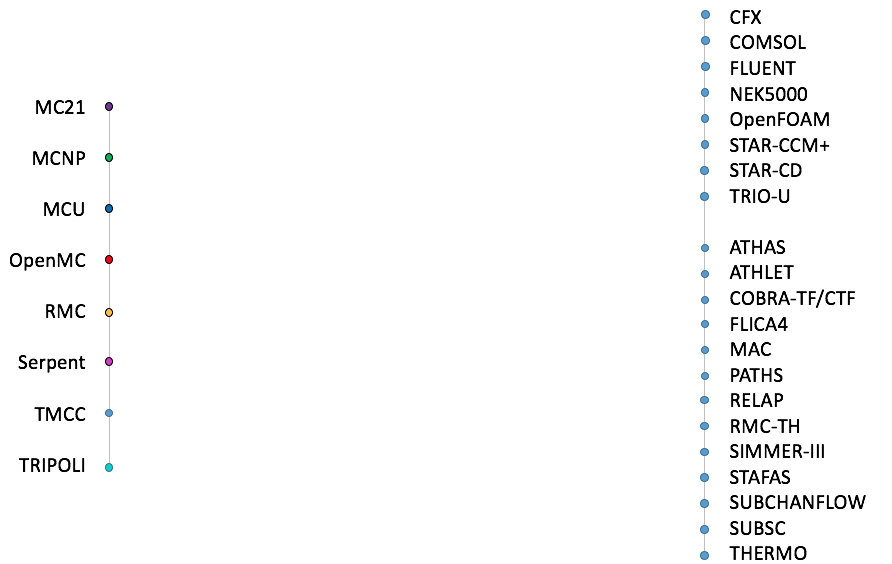
\includegraphics[width=10cm]{../Figures/history1.png}
\onslide<2>\centering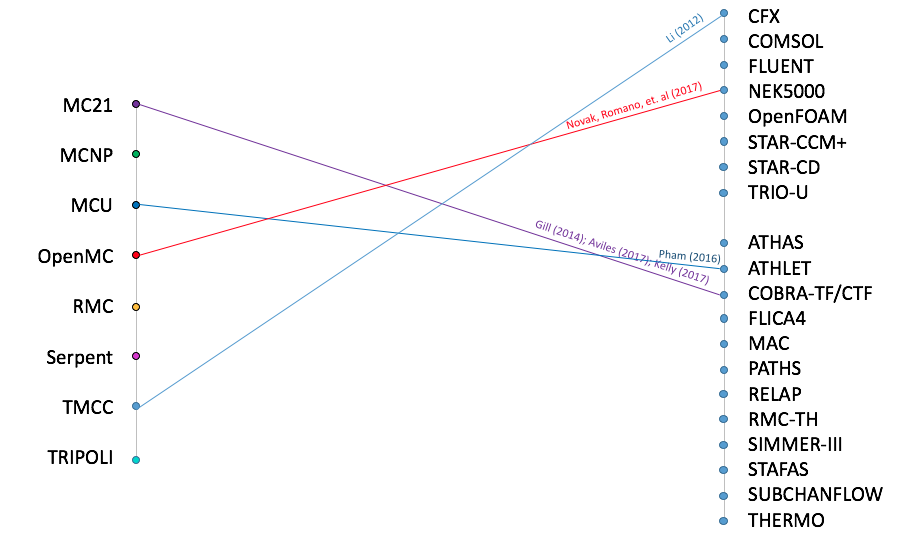
\includegraphics[width=10cm]{../Figures/history2.png}
\onslide<3>\centering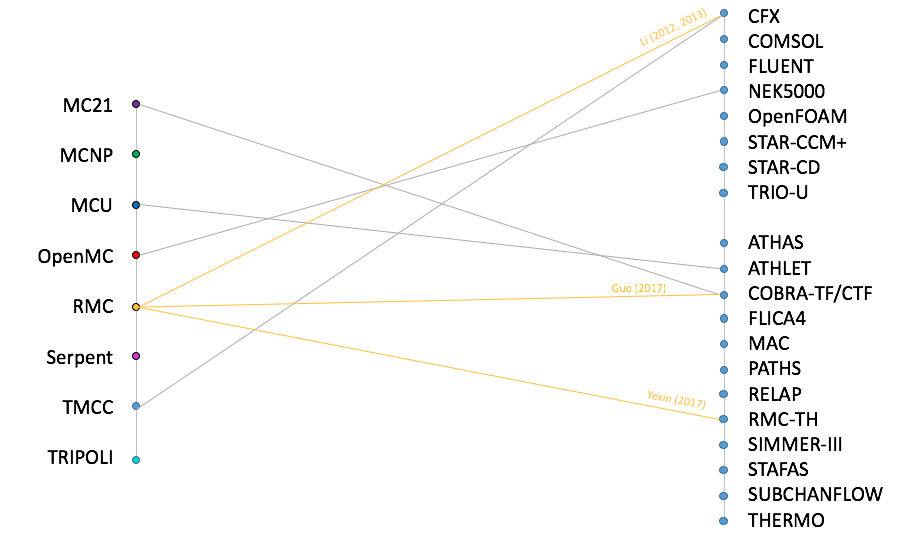
\includegraphics[width=10cm]{../Figures/history3.png}
\onslide<4>\centering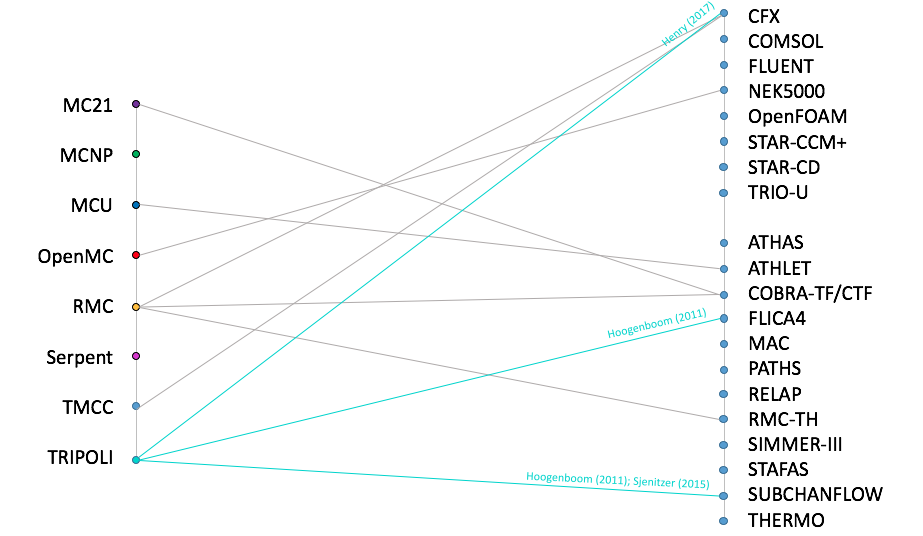
\includegraphics[width=10cm]{../Figures/history4.png}
\onslide<5>\centering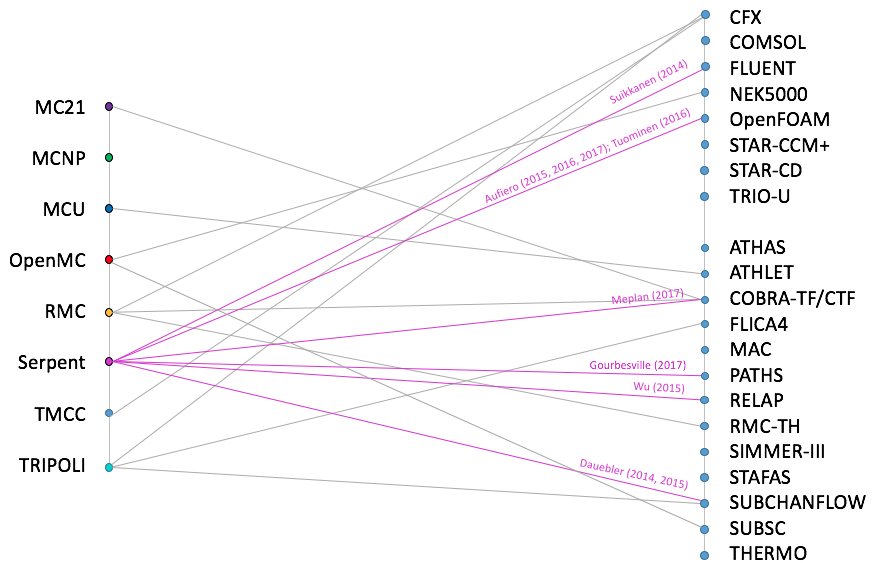
\includegraphics[width=10cm]{../Figures/history5.png}
\onslide<6>\centering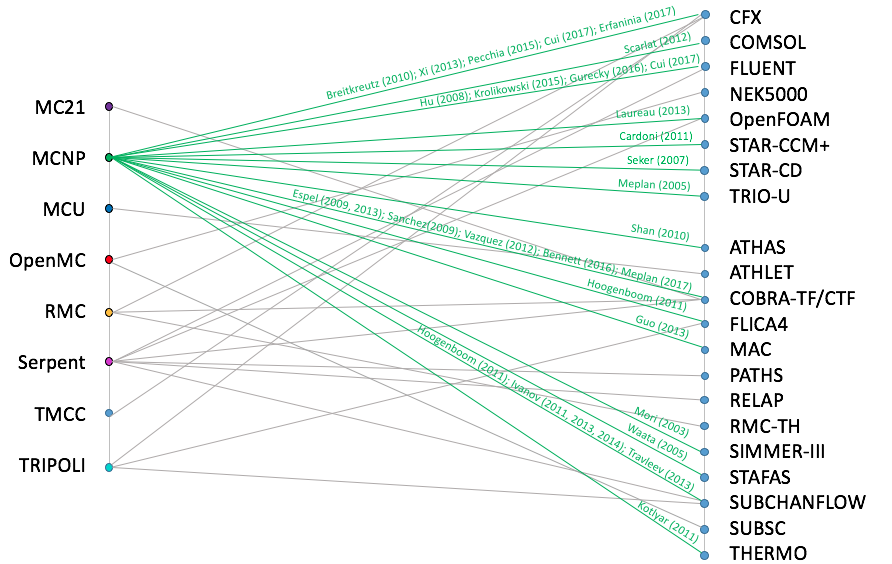
\includegraphics[width=10cm]{../Figures/history8.png}
\onslide<7>\centering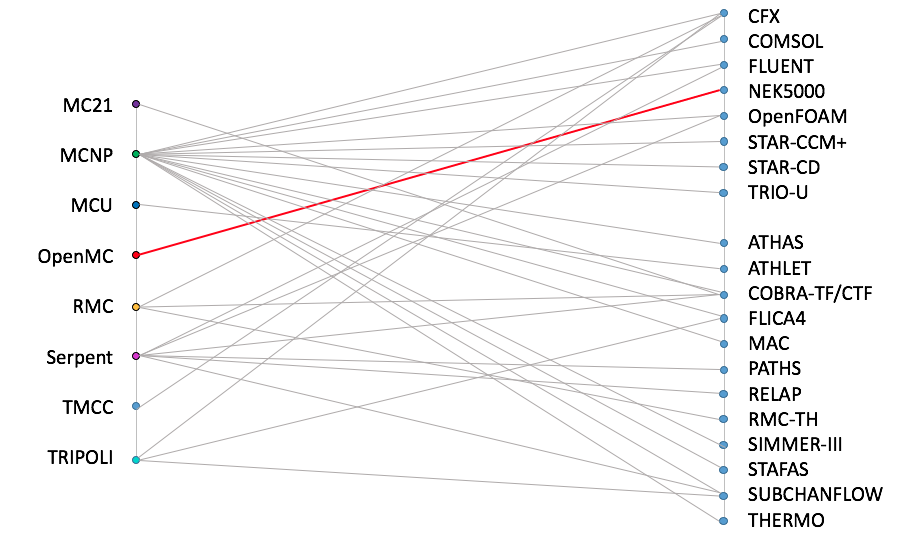
\includegraphics[width=10cm]{../Figures/history7.png}
\end{overprint}
\end{frame}

\begin{frame}{Neutronics-Thermal/Hydraulics Multiphysics}

\begin{equation}
\Sigma=\sigma(T) N(\rho)
\end{equation}
\vspace{0.5cm}
\begin{itemize}
\item Monte Carlo (MC) neutron transport
	\begin{itemize}
	\item OpenMC: {\tt https://github.com/mit-crpg/openmc}\newline
	\end{itemize}
\item Computational Fluid Dynamics (CFD) - Navier-Stokes with turbulence
	\begin{itemize}
	\item Nek5000: {\tt https://github.com/Nek5000}
	\end{itemize}
\end{itemize}
\end{frame}

\section{Software Design}

\begin{frame}{Software Design}

\begin{figure}
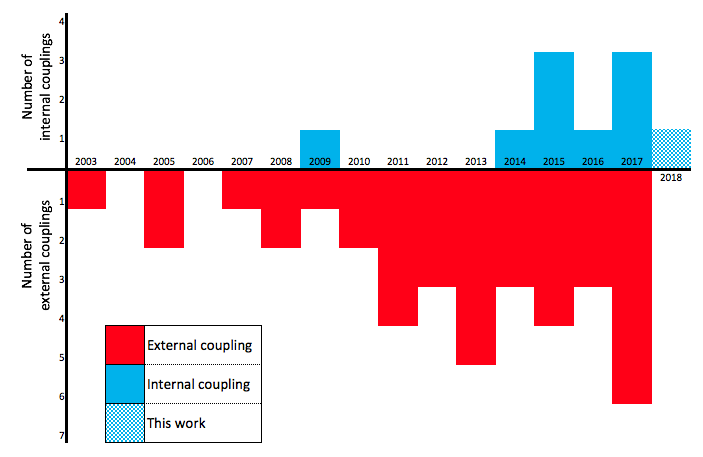
\includegraphics[width=5.65cm]{../Figures/internal_vs_external.png}
\caption{Internal and external data transfer implementations for 46 MC-T/H publications}
\end{figure}

\begin{columns}[t]
\begin{column}{0.485\linewidth}
\color{red}\textbf{External coupling}\color{black}:
	\begin{itemize}
	\item File-based communication
	\item Controlled by scripts
	\item No source code modifications required
	\item Code-specific\newline
	\end{itemize}
\end{column}
\begin{column}{0.485\linewidth}
\color{cyan}\textbf{Internal coupling}\color{black}:
	\begin{itemize}
	\item Memory-based communication
	\item Controlled by driver program
	\item Possible significant source code modifications
	\item Mostly code agnostic; re-usable
	\end{itemize}
\end{column}
\end{columns}
\end{frame}

\begin{frame}{Software Design}
\begin{figure}

\includegraphics[width=6cm]{../Figures/Moose_Multiphysics.png}
\end{figure}
\begin{itemize}
\item Multiphysics Object-Oriented Simulation Environment (MOOSE) is selected as the driver program
	\begin{itemize}
	\item Finite element framework for performing multiphysics simulations
	\item {\tt https://github.com/idaholab/moose}
	\end{itemize}
\end{itemize}
\end{frame}

\begin{frame}{Software Design}
\begin{itemize}
\item OpenMC and Nek5000 are built as dynamic libraries
\item Call OpenMC and Nek5000 routines from within MOOSE applications
\end{itemize}
\begin{figure}
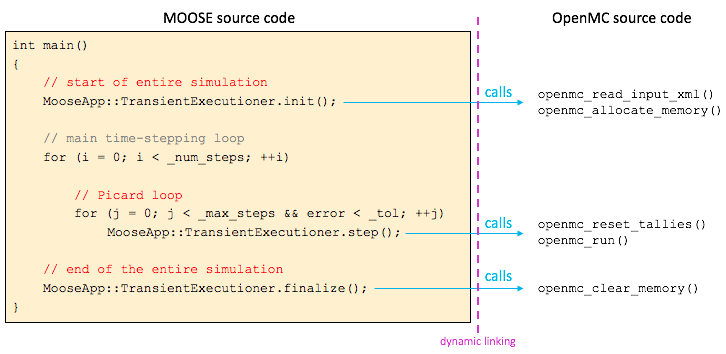
\includegraphics[width=9cm]{../Figures/moose_driver.png}
\caption{Simplified description of MOOSE-wrapped OpenMC}
\end{figure}
\end{frame}

\begin{frame}{Software Design}
\begin{itemize}
\item (Possibly) first in-memory coupling of MC and CFD codes using a third-party driver framework
\end{itemize}

\begin{figure}
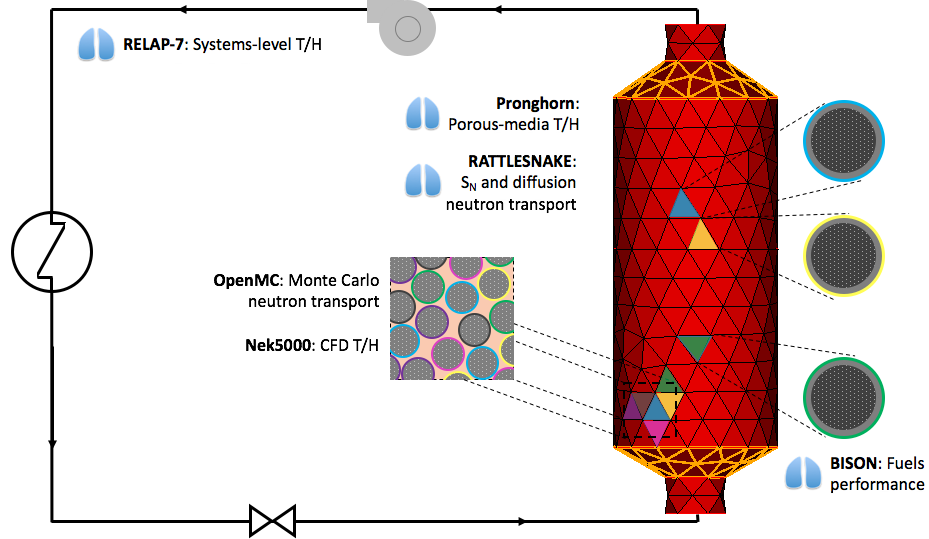
\includegraphics[width=10cm]{../Figures/MOOSE_capabilities.png}
\caption{Multiscale multiphysics coupling capabilities}
\end{figure}
\end{frame}

\begin{frame}{Okapi - {\tt https://github.com/aprilnovak/Okapi}}

\begin{figure}
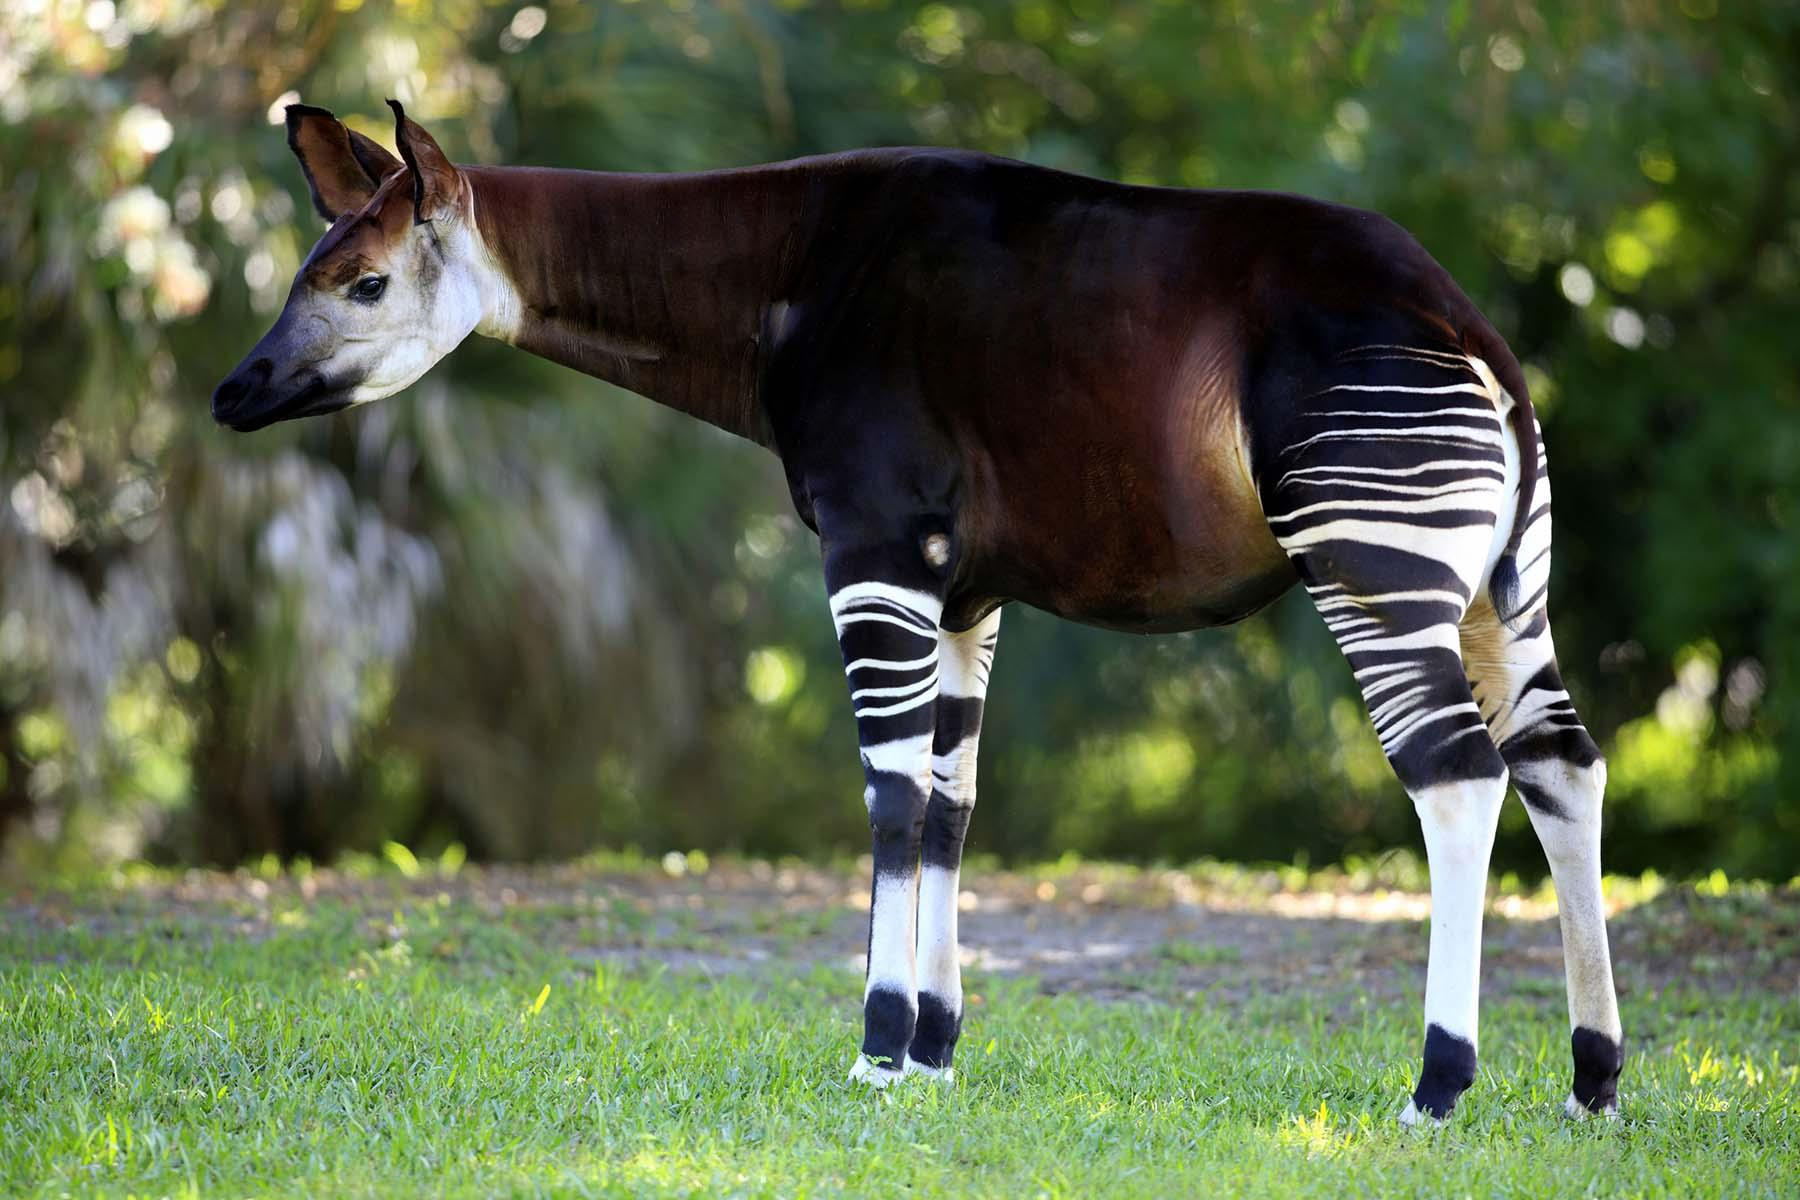
\includegraphics[width=9cm]{../Figures/okapi_animal.jpg}
\end{figure}

\centering
Okapi = OpenMC wrapped as a MOOSE application
\end{frame}

\begin{frame}{Giraffe}

\begin{figure}
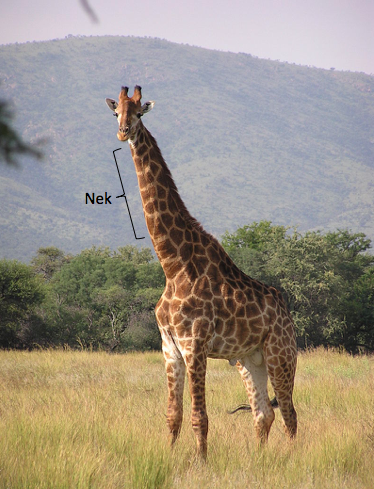
\includegraphics[width=5cm]{../Figures/giraffe_nek.png}
\end{figure}

\centering
Giraffe = Nek5000 wrapped as a MOOSE application
\end{frame}

\section{Monte Carlo \(\rightarrow\) T/H Data Transfer}

\begin{frame}{A Fundamental Difficulty}

\begin{columns}
\begin{column}{0.575\linewidth}
\vspace{0.8cm}
\begin{enumerate}
\item How to construct a mapping?\newline
\item How to limit information loss?
\end{enumerate}
\vspace{1.2cm}
\begin{figure}
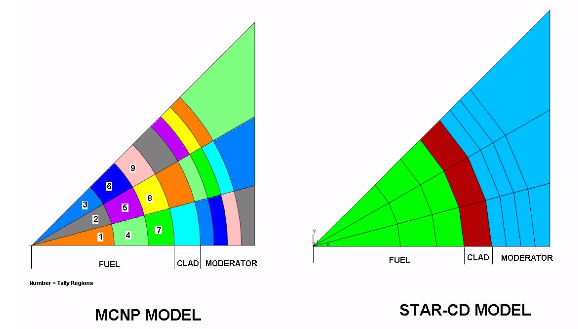
\includegraphics[width=5.5cm]{../Figures/MCNP_STARCD_meshes.png}
\caption{One-to-one correspondence between Monte Carlo and CFD cells; 3,328 cells and tallies in fuel \cite{cardoni}}
\end{figure}

%\vspace{.5cm}
\end{column}
\begin{column}{0.4\linewidth}
\begin{figure}
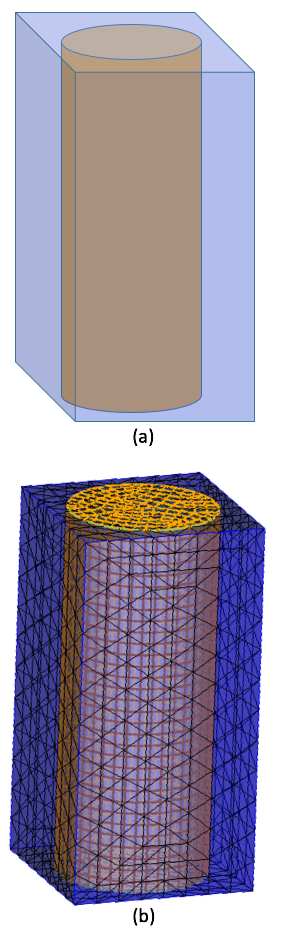
\includegraphics[width=2cm]{../Figures/MC_vs_CFD_mesh.png}
\caption{(a) Monte Carlo and (b) CFD geometry representations}
\end{figure}
\end{column}
\end{columns}

\end{frame}

\begin{comment}
\begin{frame}{Monte Carlo \(\rightarrow\) T/H Data Transfer}
Monte Carlo tallies are volume-averaged; a fission power tally is computed as:

\begin{equation}
\int_{V}F(\vv{r})\ dV
\end{equation}

where \(F\) is the fission power, \(V\) is the tally region volume, and \(\vv{r}\) is the spatial coordinate.

\end{frame}
\end{comment}

\begin{frame}{Functional Expansion Tallies (FETs)}
Spatial dependence in tallies can be obtained by tallying the coefficients of an orthogonal expansion function:

\begin{equation}
F(\vv{r})=\sum_{l=0}^{L}\sum_{m=0}^M\sum_{n=0}^NC_{lmn} P_l(x)P_m(y)P_n(z)
\end{equation}

Apply orthogonality condition:

\begin{equation}
C_{lmn}=\int_{-1}^1\int_{-1}^1\int_{-1}^1P_l(x)P_m(y)P_n(z)F(\vv{r})\ dx\ dy\ dz
\end{equation}

\begin{itemize}
\item (Possibly) the first to use functional expansion tallies in a MC-CFD-fuels simulation
\end{itemize}

\end{frame}

\begin{comment}
\begin{frame}{A Pincell Comparison}

\begin{figure}
\centering
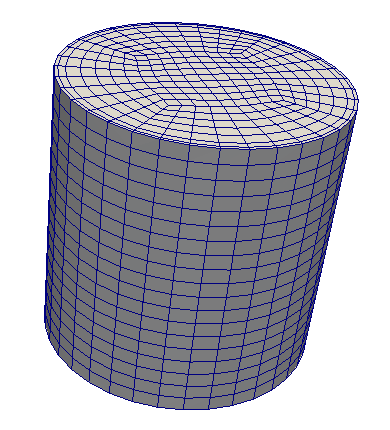
\includegraphics[width=0.2\linewidth]{../Figures/Bison_mesh.png}
\caption{Mesh for fuel rod with 6,327 cells used in the present work}
\end{figure}

\begin{table}[H]
\caption{Numbers of Monte Carlo cells and tallies in the fuel for several pincell problems}
\centering
\begin{tabular}{l c r r c}
\hline\hline
 & Year & Cells & Tallies & Bins/tally\\ [0.5ex]
\hline
MCNP/STAR-CD \cite{seker} & 2007& \hfill108 & \hfill108 & 1\\
MCNP/STAR-CCM+ \cite{cardoni}& 2011& \hfill3328 & \hfill3328 & 1\\
MCNP/FLUENT \cite{gurecky}& 2016 & \hfill14776 & \hfill14776 & 1\\
\color{cyan}OpenMC/Nek5000 & \color{cyan}2018\color{black} & \color{cyan}\hfill1\color{black} & \color{cyan}\hfill1\color{black} & \color{cyan}depends on order\color{black}\\
\hline
\end{tabular}
\vspace{1cm}
\end{table}

\end{frame}
\end{comment}

\section{T/H \(\rightarrow\) Monte Carlo Data Transfer}

\begin{frame}{T/H \(\rightarrow\) Monte Carlo Data Transfer}
With surface tracking, sample a distance \(d\) to collision for current material with where \(\xi\in(0,1]\):

\begin{subequations}
\label{eq:Sample}
\begin{eqnarray}
\xi&=&\int_0^d\Sigma_t(x)\exp{\left(-\int_{x_0}^x\Sigma_t(x')dx'\right)}dx\\
d&=&\frac{-\ln{(\xi)}}{\Sigma_t}
\end{eqnarray}
\end{subequations}

\vspace{0.25cm}
\begin{itemize}
\item At the time of writing, \(\Sigma_t(x)\) is constant in each cell, but have since implemented a Newton method to solve Eq. \eqref{eq:Sample}a (Brown and Martin, \cite{brown_martin_direct})
\item Functional expansions have been implemented in Nek5000 and MOOSE
\item (Possibly) the first MC-T/H coupling to transfer most data with functional expansions
	\begin{itemize}
	\item Several of the Serpent-T/H couplings use a different continuous representation technique (3 out of 46)
	\end{itemize}
\end{itemize}
\end{frame}

\section{Three Other Coupling Considerations}

\begin{frame}{Other Coupling Considerations}

\begin{itemize}
\item Use standard fixed-point iteration:

\begin{subequations}
\begin{eqnarray}
\phi^{(k+1)}&=&\textbf{G}\left(T^{(k)},\rho^{(k)}\right)\\
T^{(k+1)}, \rho^{(k+1)}&=&\textbf{M}\left(\phi^{(k+1)}\right)
\end{eqnarray}
\end{subequations}
	\vspace{0.05cm}
\item Interpolate cross sections stochastically in-memory (``pseudo-materials'')
	\begin{itemize}
	\item More sophisticated Windowed Multipole Method is available
	\end{itemize}
	\vspace{0.5cm}
\item Convergence is based on relative change in fuel temperature:

\begin{equation}
\max_{i\in \text{cells}}\frac{|T_{i}^{(k+1)}-T_i^{(k)}|}{T_i^{(k)}}<5\times10^{-3}
\end{equation}
\end{itemize}
\end{frame}

\section{A Simple Monte Carlo, CFD, and Fuels Performance Example}

\begin{comment}
\begin{frame}{Neutronics, Fluids, and Fuels Multiphysics}

\begin{figure}
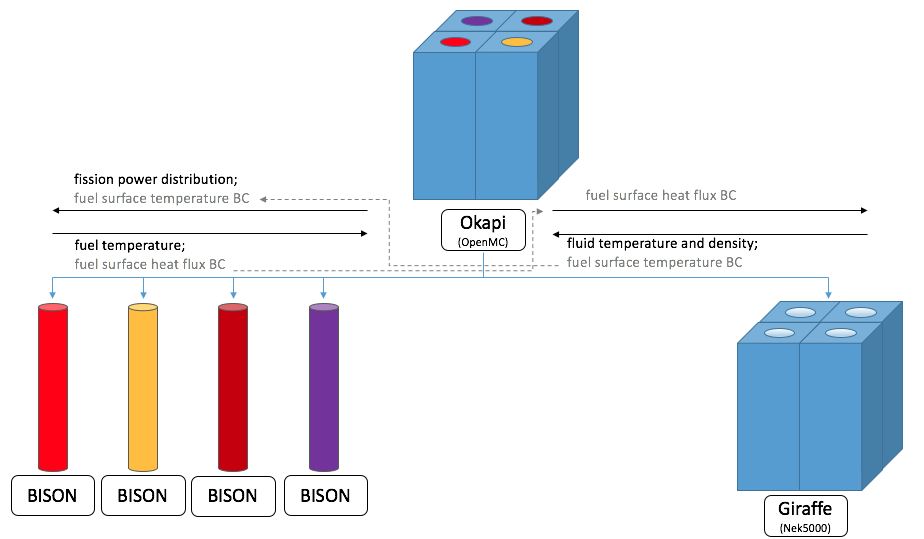
\includegraphics[width=10cm]{../Figures/hierarchy.png}
\caption{High-level description of coupled OpenMC, Nek5000, and BISON simulation}
\end{figure}

\end{frame}

\begin{frame}{Neutronics, Fluids, and Fuels Multiphysics}
\begin{figure}
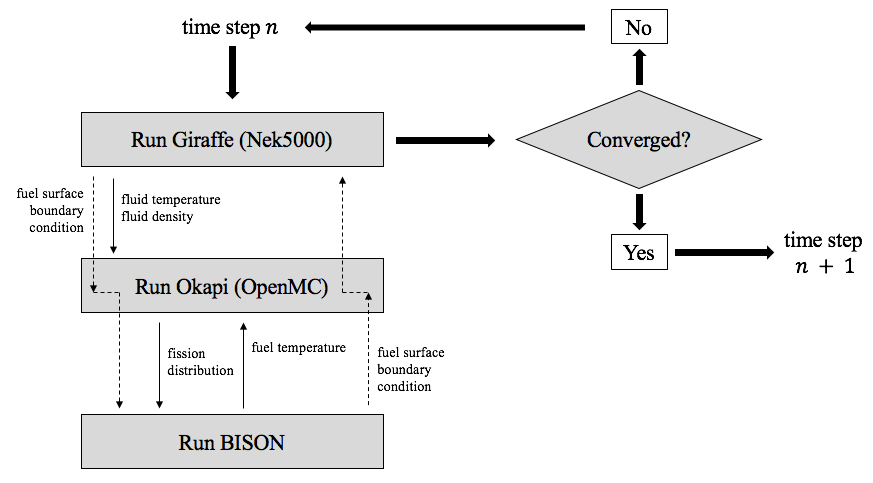
\includegraphics[width=10cm]{../Figures/runtime_design.png}
\caption{High-level description of coupled OpenMC, Nek5000, and BISON simulation}
\end{figure}
\end{frame}
\end{comment}

\begin{frame}{A Pincell Example}
\begin{columns}
\begin{column}{0.45\linewidth}
\begin{figure}
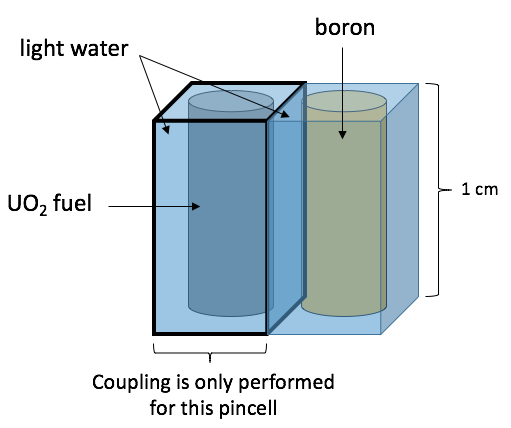
\includegraphics[width=5cm]{../Figures/pincell_picture.png}
\caption{Coupling geometry}
\end{figure}
\end{column}
\begin{column}{0.525\linewidth}
\begin{itemize}
\item OpenMC (neutron transport)
	\begin{itemize}
	\item Reflective, all sides\newline
	\end{itemize}
\item Nek5000 (incompressible Navier-Stokes, no turbulence):
	\begin{itemize}
	\item Specified pin surface heat flux
	\item Inlet 1 m/s, 550 K\newline
	\end{itemize}
\item Buffalo, a lightweight surrogate for BISON (heat conduction):
	\begin{itemize}
	\item Specific pin surface temperature
	\item Insulated top and bottom
	\end{itemize}
\end{itemize}
\end{column}
\end{columns}

\end{frame}

\begin{frame}{A Pincell Example}
\begin{figure}
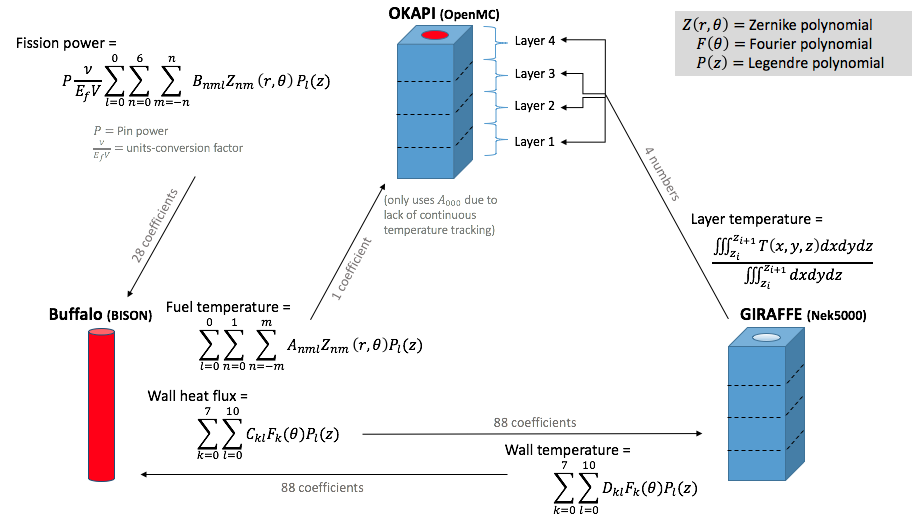
\includegraphics[width=12cm]{../Figures/detailed_coupling_pic.png}
\caption{Detailed description of coupling data transfer for simple pincell example}
\end{figure}
\end{frame}

\begin{frame}{Results}

\begin{figure}[!htb]
\centering
\begin{subfigure}{.5\textwidth}
  \centering
  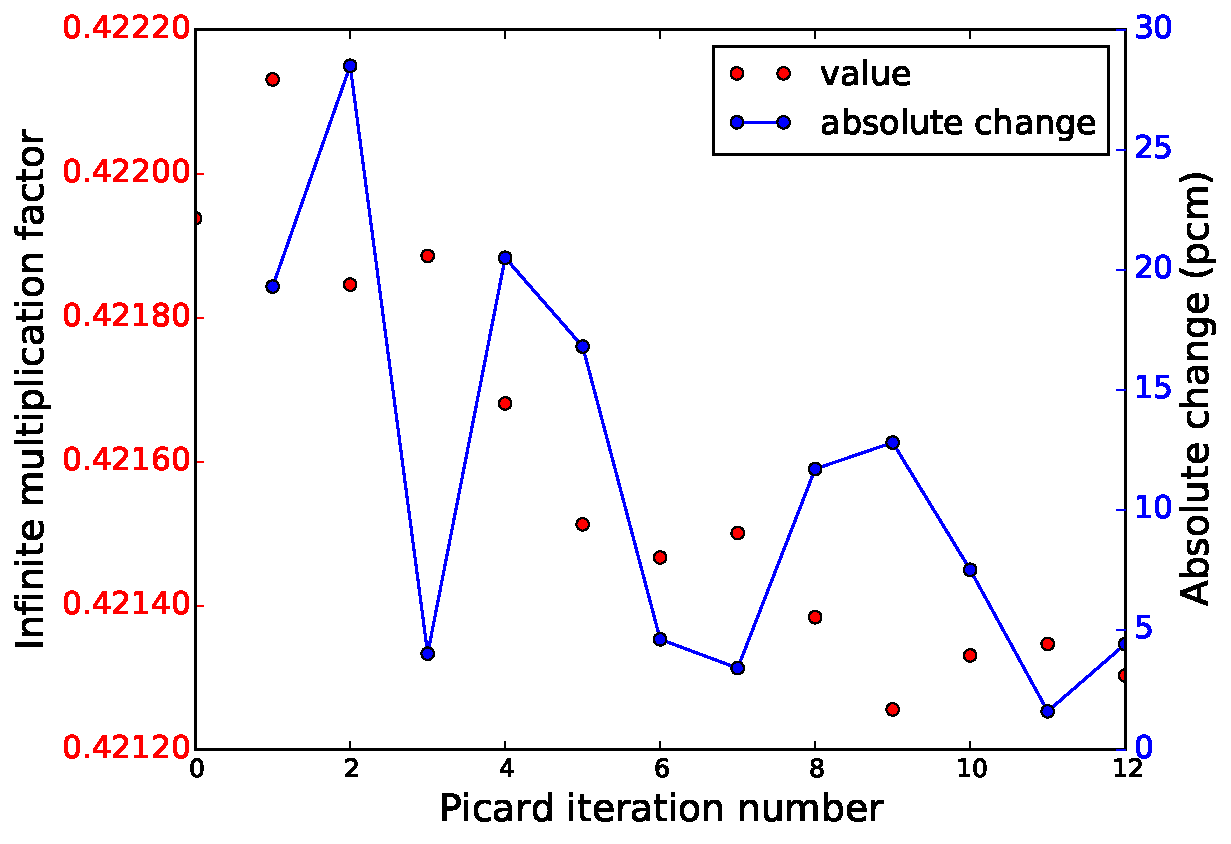
\includegraphics[width=0.9\linewidth]{../Figures/k_eff.pdf}
  \caption{\(k_{\infty}\)}
\end{subfigure}%
\begin{subfigure}{.5\textwidth}
  \centering
  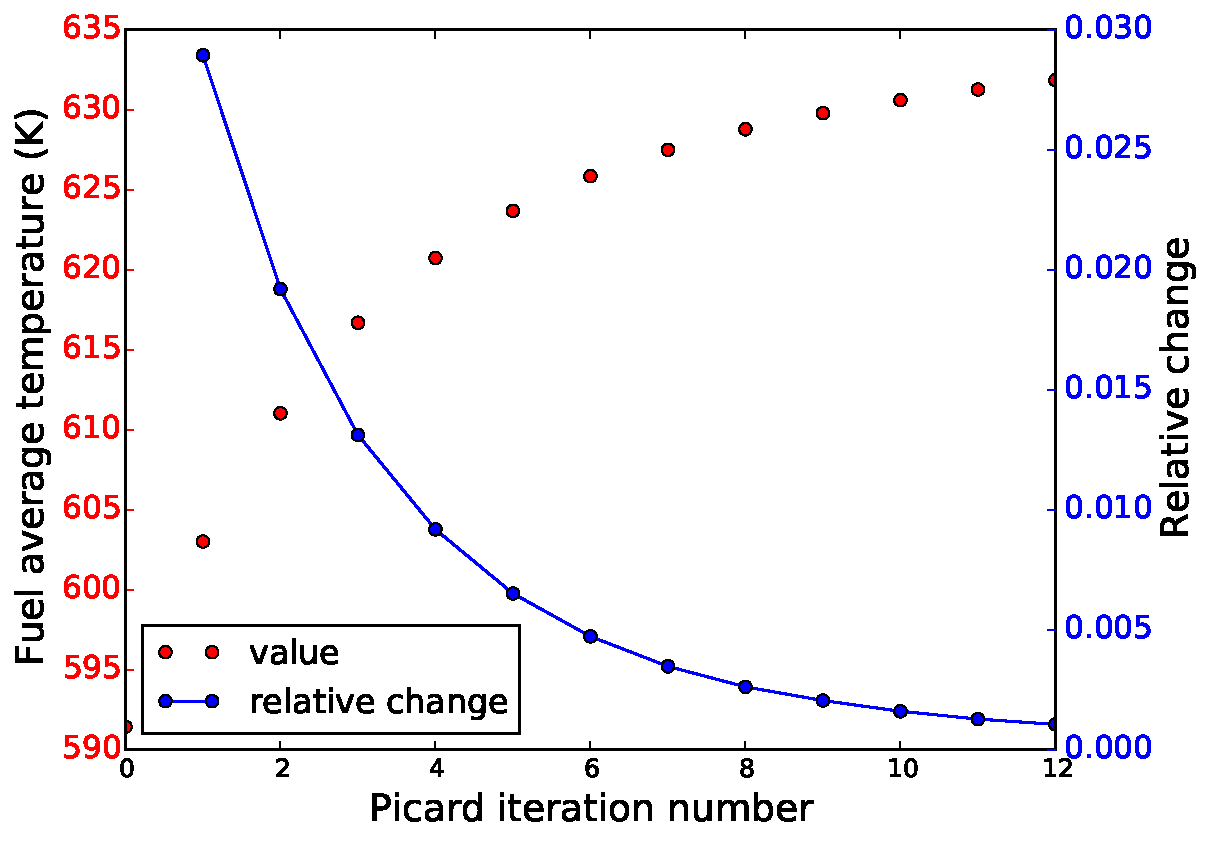
\includegraphics[width=0.9\linewidth]{../Figures/temp.pdf}
  \caption{Average fuel temperature}
\end{subfigure}
\caption{(a) \(k_{\infty}\) and (b) average
fuel temperature, with absolute and relative changes as a function of Picard iteration. The uncertainty
in \(k_{\infty}\) for each point is 0.00006.}
\end{figure}

\end{frame}

\begin{frame}{Results}
\begin{figure}[!htb]
\centering
\begin{subfigure}{.5\textwidth}
  \centering
  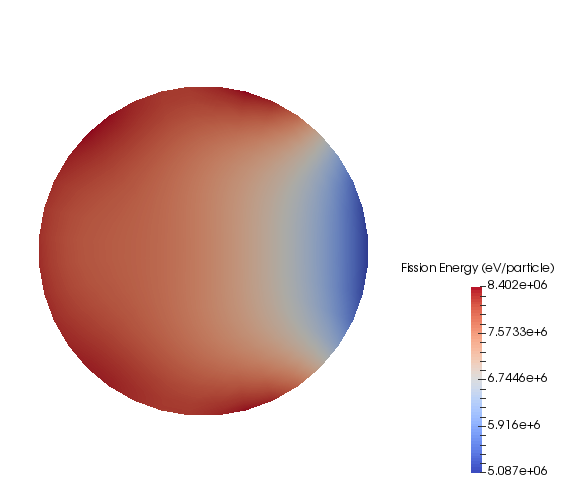
\includegraphics[width=0.9\linewidth]{../Figures/kappa_fission.png}
  \caption{Fission energy (eV/particle)}
\end{subfigure}%
\begin{subfigure}{.5\textwidth}
  \centering
  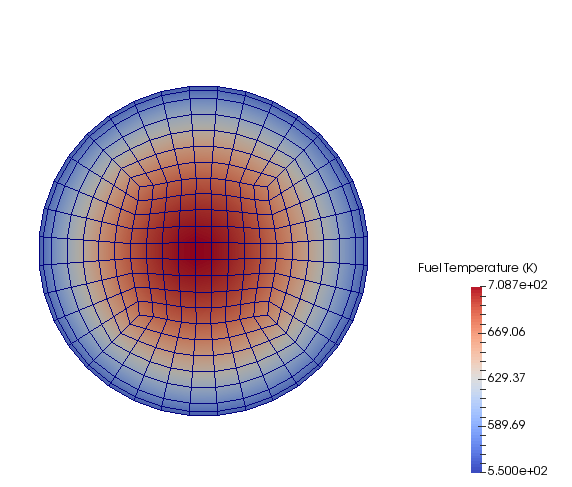
\includegraphics[width=0.9\linewidth]{../Figures/fuel_temp.png}
  \caption{Fuel temperature (K)}
\end{subfigure}
\caption{(a) Recoverable fission energy and (b)
fuel temperature}
\label{fig:openmc_buffalo}
\end{figure}
\end{frame}

\begin{frame}{Results}
\begin{figure}[!htb]
\centering
\begin{subfigure}{.5\textwidth}
  \centering
  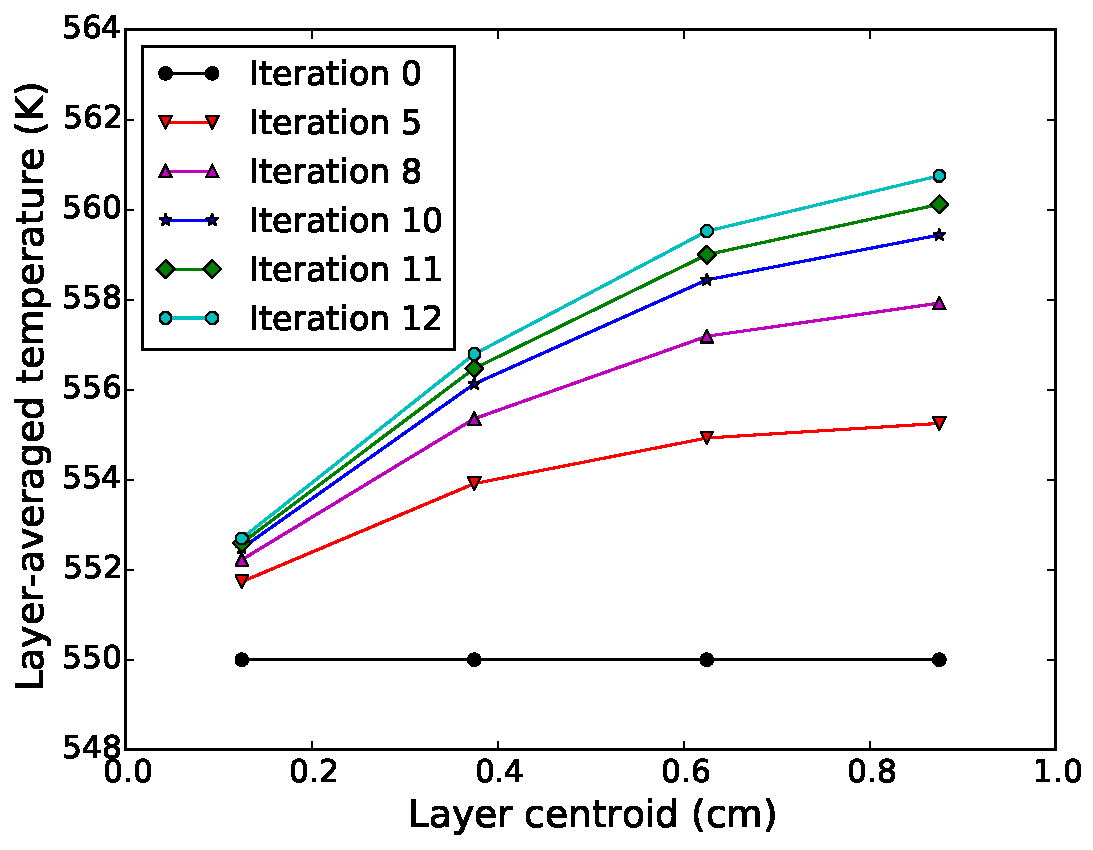
\includegraphics[width=0.8\linewidth]{../Figures/layer_temps.pdf}
  \caption{}
\end{subfigure}%
\begin{subfigure}{.5\textwidth}
  \centering
  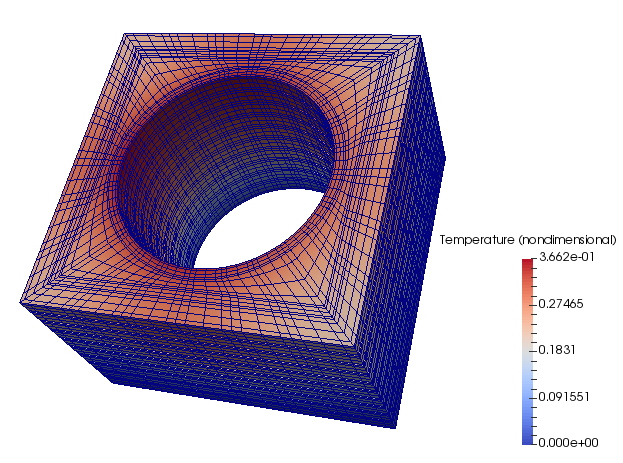
\includegraphics[width=0.9\linewidth]{../Figures/Nek_with_mesh.png}
  \caption{}
\end{subfigure}
\caption{(a) Layer-averaged fluid temperatures for several Picard iterations
and (b) (nondimensional) fluid temperature at Picard iteration 12.}
\label{fig:layer_temps}
\end{figure}
\end{frame}

\section{Conclusions}

\begin{frame}{Conclusions}
\begin{itemize}
\item In-memory coupling of Monte Carlo and CFD using an established driver framework
	\begin{itemize}
	\item Many possibilities for coupling to other MOOSE applications\newline
	\end{itemize}
\item Functional expansion tallies used for most of the data transfers
	\begin{itemize}
	\item Continuous representation of solutions
	\item Relatively few floating point number transfers\newline
	\end{itemize}
\item Future work:
	\begin{itemize}
	\item Repeat simulations with continuous material tracking
	\item More sophisticated relaxation iterations, convergence estimates, and temperature-dependent cross sections
	\end{itemize}
\end{itemize}
\end{frame}

\begin{frame}{Author Contributions}
\begin{figure}
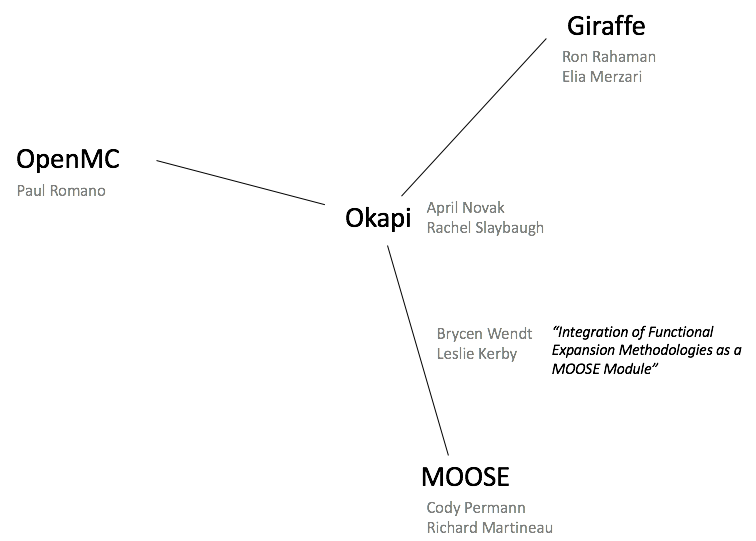
\includegraphics[width=10cm]{../Figures/work_division.png}
\end{figure}
\end{frame}

\begin{frame}
\begin{figure}
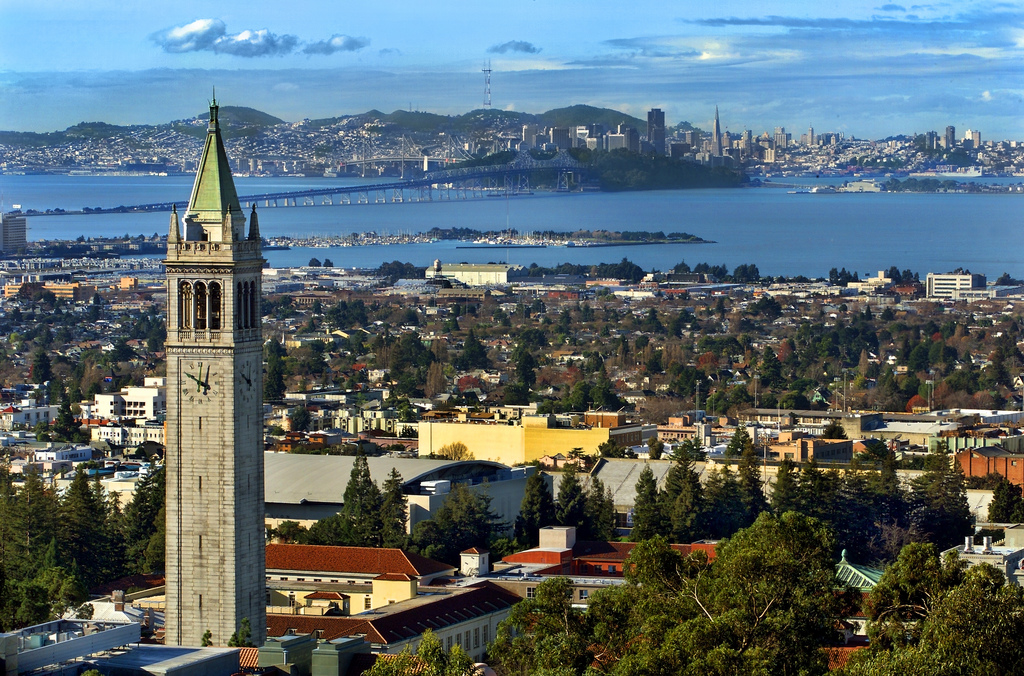
\includegraphics[width=9cm]{../Figures/berkeley.jpg}
\end{figure}
\centering
Thank you!

% to get all of the references to populate the bibliography
\footnotesize
\color{white}\cite{mori,waata,seker,espel,sanchez,cardoni,ivanov,travleev,espel_2013,ivanov_2013,daeubler,ivanov_2014,daeubler_2015,henry,aviles,li_2013,suikkanen,wu,hu,vazquez,meplan,aufiero,aufiero_2017,krolikowski,aufiero_2016,pham,novak,guo,scarlat,yexin,gurecky,sjenitzer,breitkreutz,gill,erfaninia,bennett,gourbesville,guo_2013,hoogenboom,kelly,laureau,smure,pecchia,shan,li_2012,kotlyar_2011}
\color{black}
\end{frame}

\appendix

\begin{frame}[allowframebreaks]
\footnotesize
\bibliographystyle{unsrt}
\bibliography{physor}
\end{frame}

\end{document}
